\begin{tikzpicture}[scale=1.3]
  \foreach \i in {0,...,4} {
    \coordinate (P\i) at ({90+72*\i}:1);
  }
  \draw[thick, blue] (P0) -- (P1) -- (P2) -- (P3) -- (P4) -- cycle;
  \foreach \i in {0,...,4} { \fill[blue] (P\i) circle (1pt); }
  \fill (0,0) circle (1pt) node[below left, font=\small] {$z$};
  % rotation by 2pi/n
  \draw[->, red, thick] (0.35,0) arc[start angle=0, end angle=72, radius=0.35];
  \node[red, font=\small] at (0.62,0.38) {$\tfrac{2\pi}{n}$};
  % a flip axis through a vertex and the opposite edge midpoint
  \draw[dashed, purple] (0,1.35) -- (0,-1.25);
  \node[purple, font=\small, align=center] at (0,-1.65) {flip: $180^\circ$ rotation\\about an axis in the $xy$-plane};
\end{tikzpicture}
